\section{Internal Tests}

\subsection{GOAL Test Set}
First of all, let us how many unsuccessful complementation tasks there were with the internal tests on the \goal{} test set. Table~\ref{i.g.out_table} shows the number of timeouts and memory excesses for each of the eight tested versions of the Fribourg construction.

\begin{table}[ht]
\centering
% latex table generated in R 3.1.2 by xtable 1.7-4 package
% Sat Jun  6 16:42:17 2015
\begin{tabular}{lrr}
  \hline
Construction & Timeouts & Memory excesses \\ 
  \hline
Fribourg & 48 & 0 \\ 
  Fribourg+R2C & 30 & 0 \\ 
  Fribourg+R2C+C & 54 & 0 \\ 
  Fribourg+M1 & 2 & 0 \\ 
  Fribourg+M1+M2 & 1 & 0 \\ 
  Fribourg+M1+R2C & 1 & 0 \\ 
  Fribourg+M1+R2C+C & 8 & 0 \\ 
  Fribourg+R & 48 & 0 \\ 
   \hline
\end{tabular}

\caption{Number of timeouts and memory excesses in the internal tests on the \goal{} test set.}
\label{i.g.out_table}
\end{table}

As we can see in the table, there were no memory excesses, that is, none of the 11,000 complementation tasks required more than 1 GB memory (actually, Java heap size). On the other hand, there is quite a number of timeouts. If we extract the effective samples from these result sets, we get a set of 10,939 automata. That means that these 10,939 automata have been successfully completed by all the versions of the Fribourg construction, whereas the remaining 61 automata (0.55\%) provoked a timeout in at least one of the versions.

Our main analysis is now about the sizes of the complements of these 10,939 automata. With size we mean the number of states of an automaton. A stripchart as the one in Figure~\ref{i.g.stripchart} is a good way to get a first glance of the complement sizes. Each horizontal strip contains 10,939 dots, each one corresponding to a produced complement automaton. The x-position of a dot indicates the size of the corresponding complement automaton.

\begin{figure}[ht]
\centering
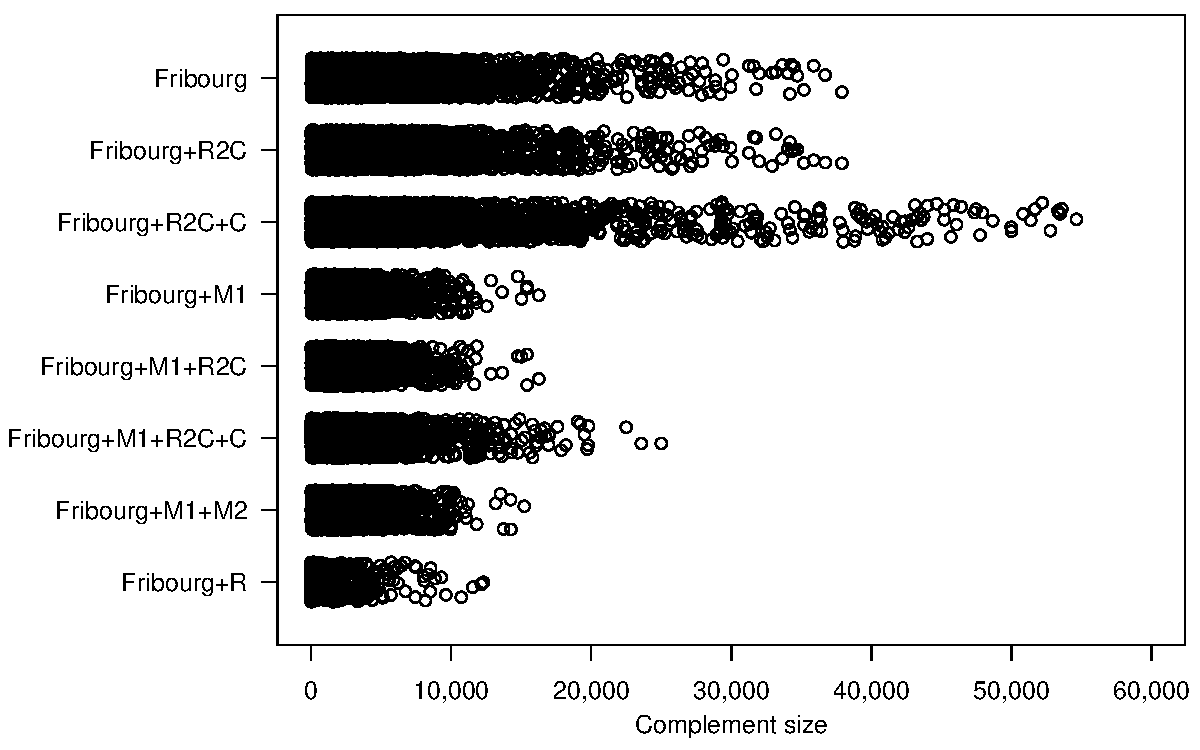
\includegraphics[width=0.7\textwidth]{figures/r/internal/goal/s.stripchart.pdf}
\caption{Stripchart with the complement sizes of the 10,939 effective samples of the \goal{} test set.}
\label{i.g.stripchart}
\end{figure}

The first thing to note is that the distribution of complement sizes is extremely right-skewed (also known as positive-skewed). The peak close to the left end of the x-axis and there is a long tail toward the right. This means that most of the complements are very small and the frequency decreases with increasing complement size. Finally, there are some few complements which are very large. This distribution implies that the mean is generally higher than the median, because the mean is ``dragged'' to the right by the few very large complements.

Next, we can compare the distributions of the individual version to each other. While Fribourg and Fribourg+R2C have a similarly long tail, Fribourg+R2C+C has a considerably longer one. This clearly is the effect of increasing the size of 91\% of the automata by adding a sink state in order to make them complete. Next, Fribourg+M1, Fribourg+M1+M2, and Fribourg+M1+R2C have similarly long tails that are significantly shorter than the ones of the previous versions. This indicates that the M1 optimisation is effective in reducing the size of otherwise large complements. Fribourg+M1+R2C+C, as expected, again increases the size of the tail due to the C option. Finally, Fribourg+R has a very short tail and an even higher concentration of very small complements. This is because the complements are pruned by removing their unreachable and dead states, and thus at least the complements of the 61.8\% universal input automata are reduced to empty automata of size 1.

Having a first impression of the distribution of complement sizes, we can look at some statistics characterising this distribution. Table~\ref{i.g.stats_table} shows the mean complement size along with the classic five-number summary consisting of minimum value, 25th percentile, median, 75th percentile and maximum value for each version of the Fribourg construction. As expected, the mean is always higher than the median. Generally, the median is a more robust metrics than the mean, because it is not affected by the value of outliers. This applies specifically to our distribution where some few very large complements might significantly increase the man whereas they leave the median unaffected. Therefore, the median will be our main metric, and the subsequent analyses will be based on the median.

\begin{table}[ht]
\centering
% latex table generated in R 3.1.2 by xtable 1.7-4 package
% Sat Jun  6 16:42:20 2015
\begin{tabular}{lrrrrrr}
  \hline
Construction & Mean & Min. & P25 & Median & P75 & Max. \\ 
  \hline
Piterman+EQ+RO & 209.6 & 1 & 38.0 & 80.0 & 183.0 & 20,349 \\ 
  Slice+P+RO+MADJ+EG & 949.4 & 2 & 120.0 & 396.0 & 1,003.0 & 41,081 \\ 
  Fribourg+M1+R2C & 1,017.3 & 2 & 153.0 & 452.0 & 1,134.0 & 37,068 \\ 
   \hline
\end{tabular}

\caption{Statistics of the complement sizes of the 10,939 effective samples of the \goal{} test set.}
\label{i.g.stats_table}
\end{table}

Going through the median values in Table~\ref{i.g.stats_table} we encounter some surprises. To begin with, as expected, there is a decrease from Fribourg (761) to Fribourg+R2C (689). Then, however, there is a significant drop to 451 with Fribourg+R2C+C. This is a surprise insofar as by looking at Figure~\ref{i.g.stripchart}, Fribourg+R2C+C seems to have the worst performance at a first glance. Indeed it also has the highest mean, which is due to the group of extremely large complements. The median, however, is very low, even lower than the one of Fribourg+M1 with its significantly shorter tail in Figure~\ref{i.g.stripchart}. Also the 25th percentile of Fribourg+R2C+C is with 85 one of the lowest. Going to the other side of the median, however, the 75th percentile (2,329) is the largest of all versions. A possible characterisation of this phenomenon is that the C option (together with R2C) makes small complements smaller, and large complements larger. The diminishment of small complements is far-reaching enough that the median is affected by it and decreased significantly.

The next thing we see in Table~\ref{i.g.stats_table} is that the median of Fribourg+M1 (482) is slightly lower than the median of Fribourg+M1+M2 (496). The same applies to the 25th and 75th percentile. This backs up our statement from Section~\ref{4_internal} that Fribourg+M1 performs better on the \goal{} teset set than Fribourg+M1+M2. The difference is rather small (the median increase is 2.9\%), but it is enough to consider Fribourg+M1 as the better of the two versions, and to combine it therefore with R2C and R2C+C.

Fribourg+M1+R2C brings down the median from 482 to 447, with respect to Fribourg+M1. Also the 25th and 75th percentile are decreased. Adding the C option to Fribourg+M1+R2C, again causes the median to drop dramatically, from 447 to 331. The 25th percentile decreases from 152 to 83. The 75th percentile however increases from 1,118 to 1,208.5. Here we have again the same picture of the effecto of adding the C option that we had before. Namely that small complements are made smaller, and large complements are made larger.

Finally, the last row in Table~\ref{i.g.stats_table} with Fribourg+R shows the extent of unreachable and dead states that the Fribourg construction produces. The median is 1, and a further analysis reveals that the single-state complements go up to the 61st percentile. That is, 61\% of the complements have a size of 1. This is likely to correspond to the 61.8\% of universal automata in the GOAL test set whose complements can be reduced to empty automata with a single state.


% \begin{table}[ht]
% \centering
% % latex table generated in R 3.1.2 by xtable 1.7-4 package
% Wed Aug 19 09:24:28 2015
\begin{tabular}{LrrrrrrRr}
  \hline
Construction & Mean & Min. & P25 & Median & P75 & Max. & Total & $\approx$ hours \\ 
  \hline
Fribourg & 8.5 & 2.5 & 3.3 & 4.9 & 7.3 & 586.0 & 93,351.2 & 259 \\ 
  Fribourg+R2C & 6.6 & 2.2 & 2.9 & 4.2 & 6.4 & 219.7 & 72,545.7 & 202 \\ 
  Fribourg+R2C+C & 8.5 & 2.2 & 2.6 & 3.5 & 6.4 & 582.9 & 93,396.2 & 259 \\ 
  Fribourg+M1 & 4.9 & 2.5 & 3.2 & 4.1 & 5.9 & 55.1 & 54,061.3 & 150 \\ 
  Fribourg+M1+R2C & 4.4 & 2.2 & 2.8 & 3.6 & 5.3 & 42.5 & 48,572.0 & 135 \\ 
  Fribourg+M1+R2C+C & 5.6 & 2.5 & 3.2 & 4.0 & 6.5 & 147.4 & 60,918.9 & 169 \\ 
  Fribourg+M1+M2 & 4.6 & 2.2 & 2.9 & 3.8 & 5.1 & 38.4 & 49,848.0 & 138 \\ 
  Fribourg+R & 7.5 & 2.2 & 3.0 & 3.9 & 6.3 & 470.5 & 82,387.3 & 229 \\ 
   \hline
\end{tabular}

% \caption{Running times in seconds of the complementation tasks, measured as CPU time.}
% \end{table}
% \textcolor{red}{It is strange that Fribourg+R is so much faster than Fribourg}

\subsubsection{Statistics Split Up by dt/da classes}

\newcommand{\perspwidth}{0.475}

\begin{figure}[ht]
\centering
  \hfill
  \begin{subfigure}[t]{\perspwidth\textwidth}
  \centering
  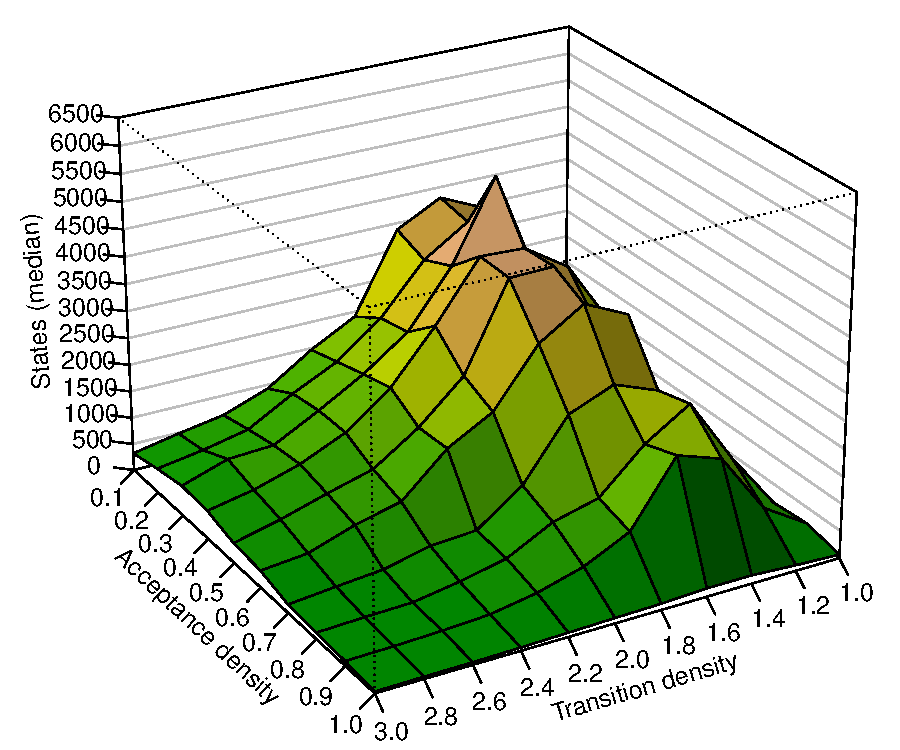
\includegraphics[width=\textwidth]{figures/r/internal/goal/s.median.Fribourg.pdf}
  \caption{Fribourg}
  \end{subfigure}
  \hfill
  \begin{subfigure}[t]{\perspwidth\textwidth}
  \centering
  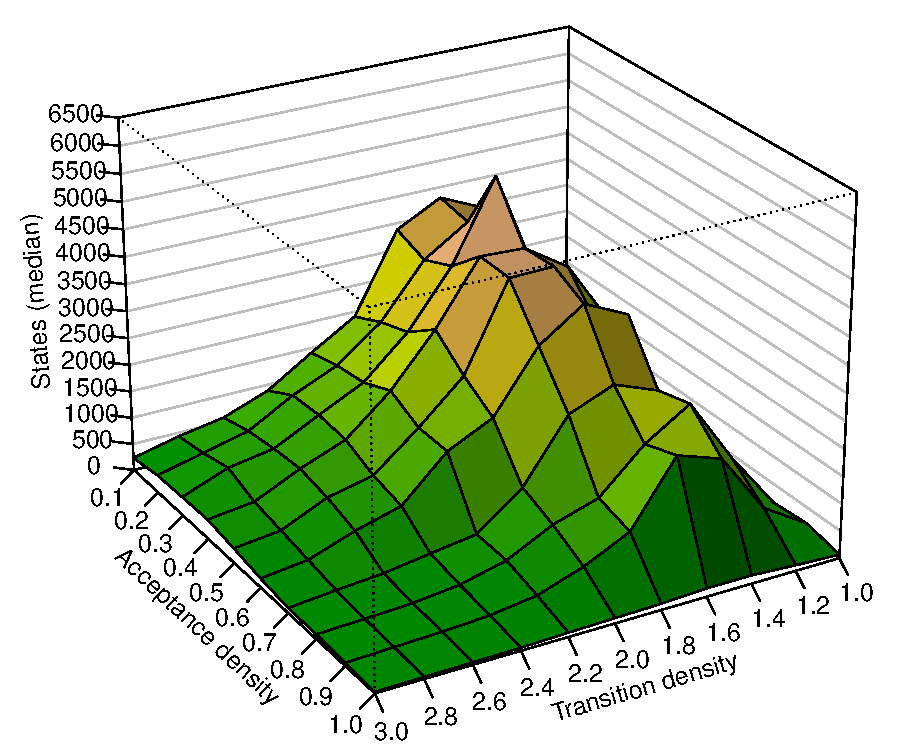
\includegraphics[width=\textwidth]{figures/r/internal/goal/s.median.Fribourg+R2C.pdf}
  \caption{Fribourg+R2C}
  \end{subfigure}
  \hfill

  \hfill
  \begin{subfigure}[t]{\perspwidth\textwidth}
  \centering
  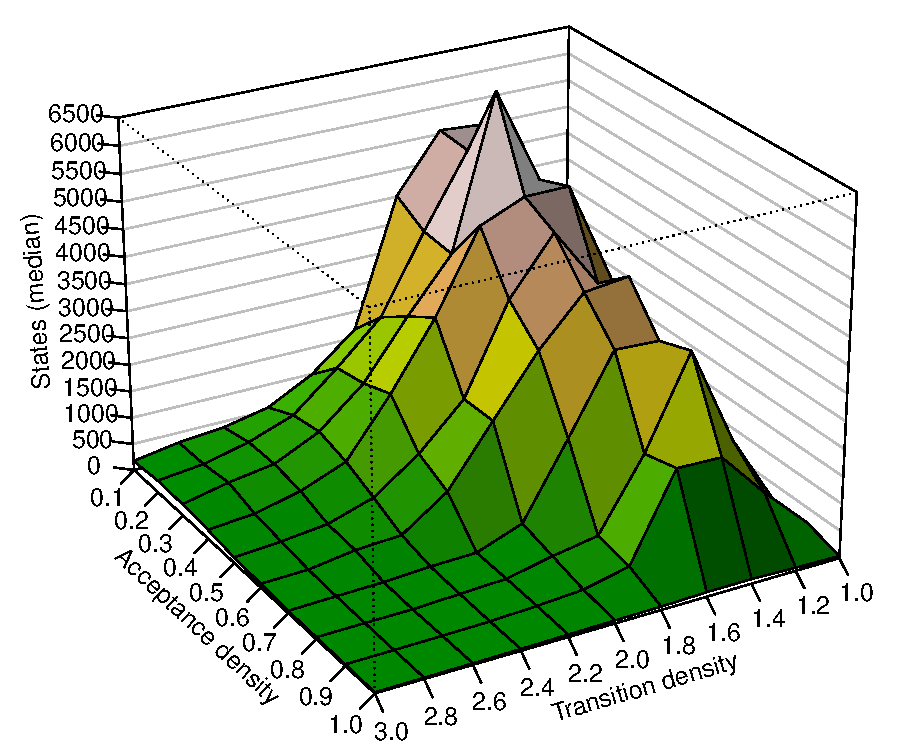
\includegraphics[width=\textwidth]{figures/r/internal/goal/s.median.Fribourg+R2C+C.pdf}
  \caption{Fribourg+R2C+C}
  \end{subfigure}
  \hfill
  \begin{subfigure}[t]{\perspwidth\textwidth}
  \centering
  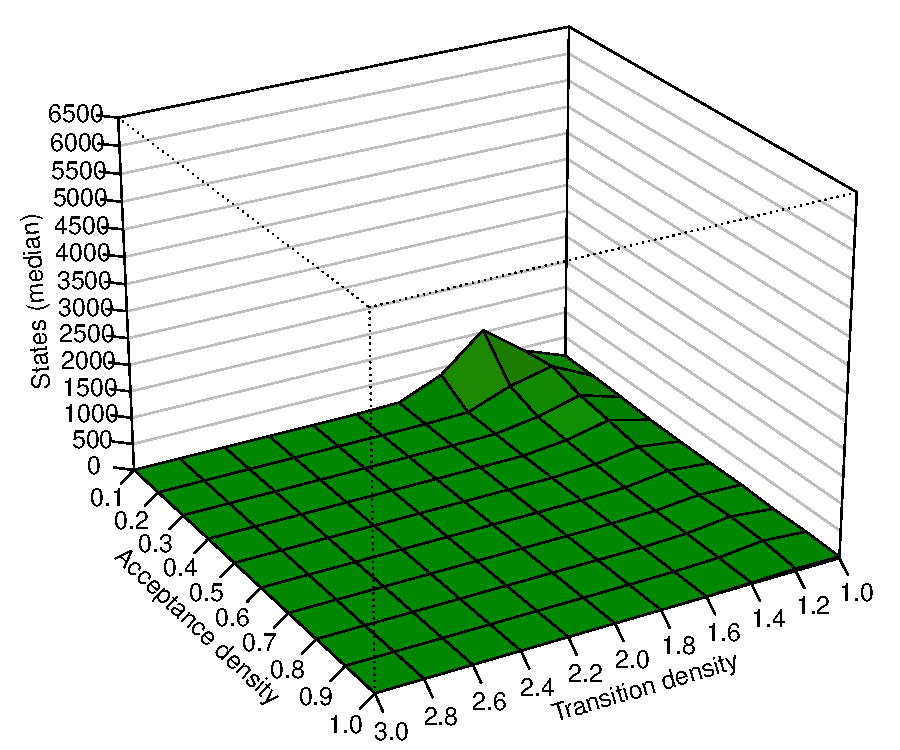
\includegraphics[width=\textwidth]{figures/r/internal/goal/s.median.Fribourg+R.pdf}
  \caption{Fribourg+R}
  \end{subfigure}
  \hfill  
\caption{Median states}
\end{figure}

\begin{figure}[ht]
\centering
  \hfill
  \begin{subfigure}[t]{\perspwidth\textwidth}
  \centering
  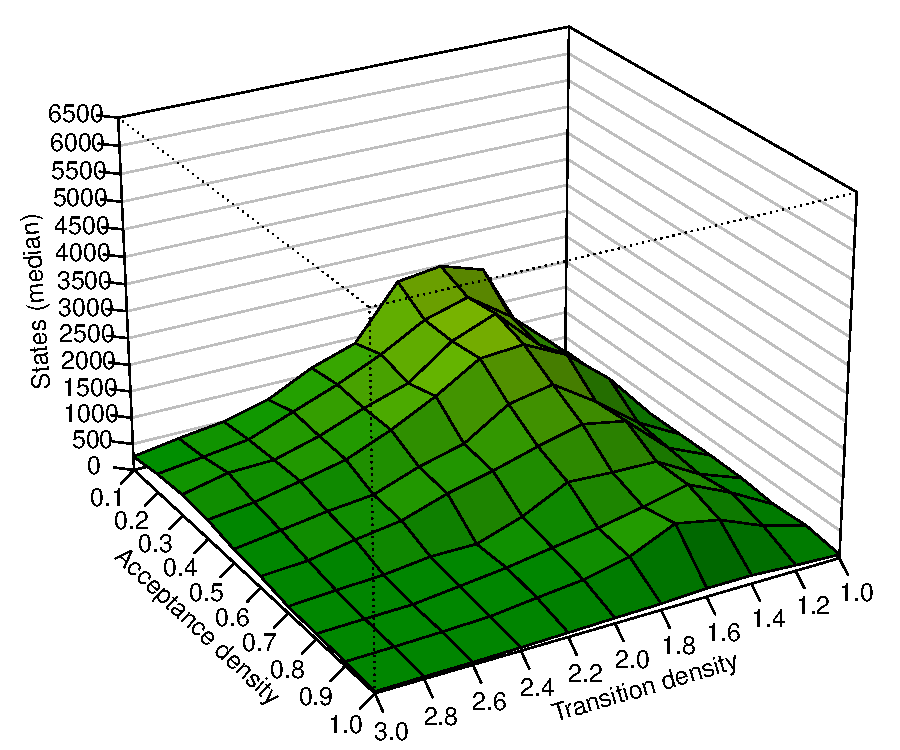
\includegraphics[width=\textwidth]{figures/r/internal/goal/s.median.Fribourg+M1.pdf}
  \caption{Fribourg+M1}
  \end{subfigure}
  \hfill
  \hfill
  \begin{subfigure}[t]{\perspwidth\textwidth}
  \centering
  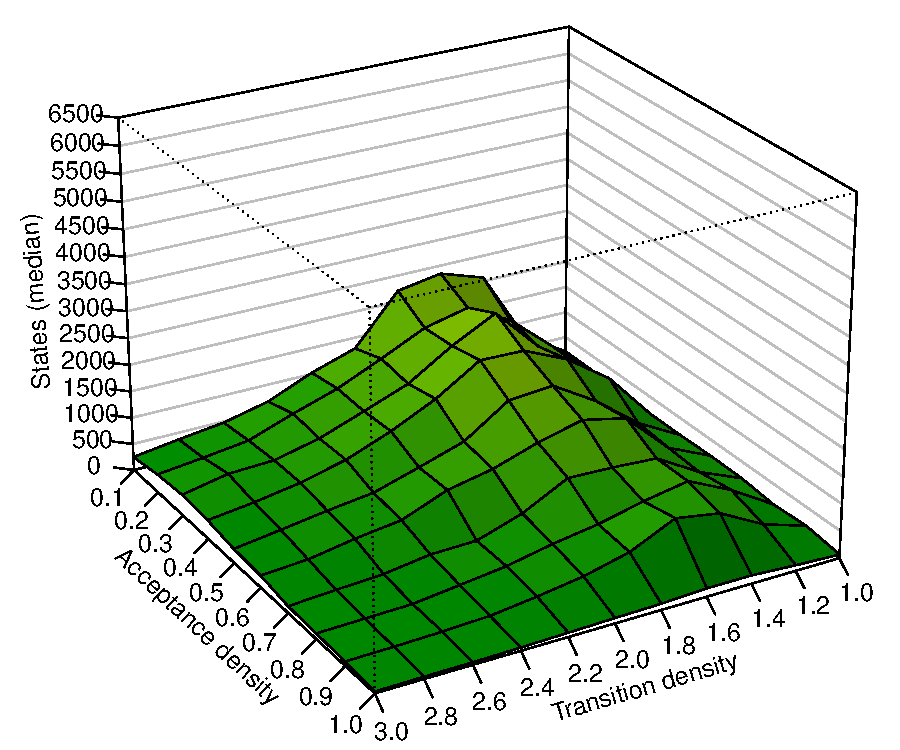
\includegraphics[width=\textwidth]{figures/r/internal/goal/s.median.Fribourg+M1+M2.pdf}
  \caption{Fribourg+M1+M2}
  \end{subfigure}
  \hfill

  \hfill
  \begin{subfigure}[t]{\perspwidth\textwidth}
  \centering
  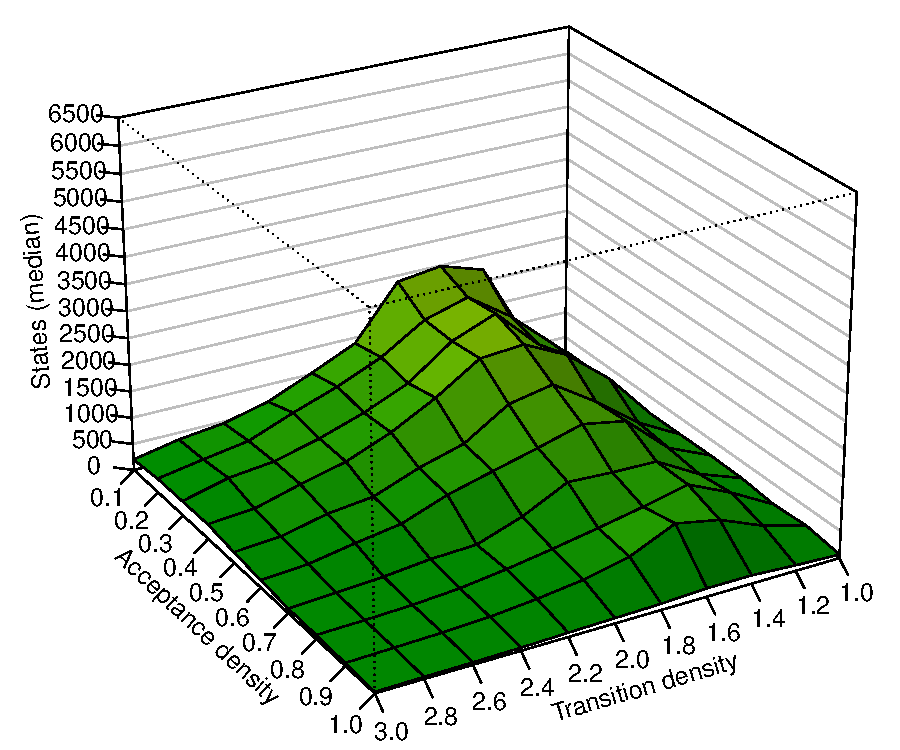
\includegraphics[width=\textwidth]{figures/r/internal/goal/s.median.Fribourg+M1+R2C.pdf}
  \caption{Fribourg+M1+R2C}
  \end{subfigure}
  \hfill
  \begin{subfigure}[t]{\perspwidth\textwidth}
  \centering
  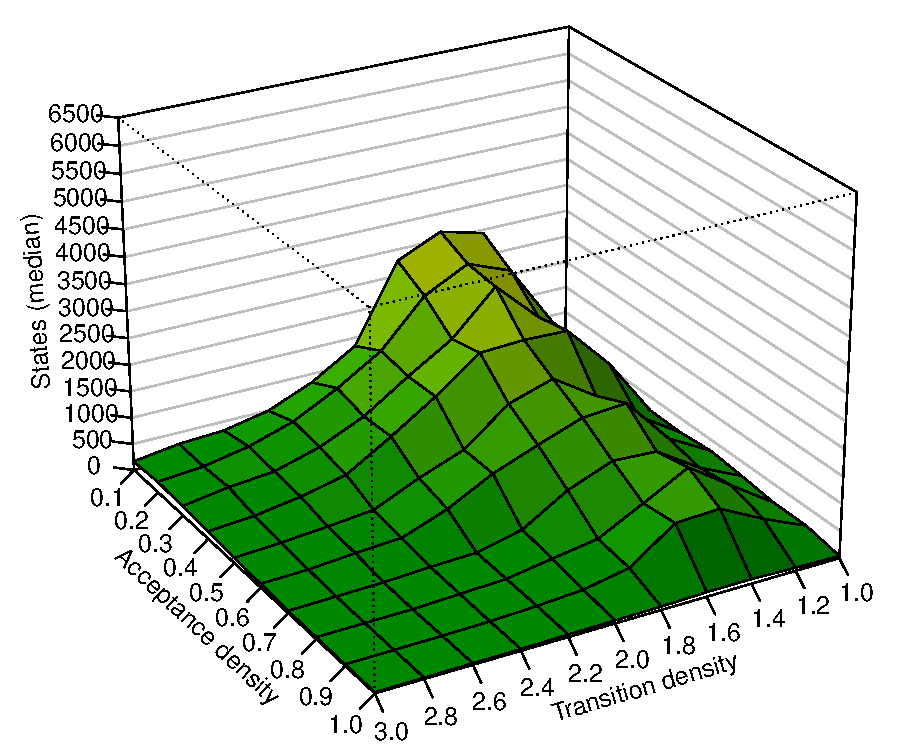
\includegraphics[width=\textwidth]{figures/r/internal/goal/s.median.Fribourg+M1+R2C+C.pdf}
  \caption{Fribourg+M1+R2C+C}
  \end{subfigure}
  \hfill
\end{figure}

\subsubsection{Difficulty Classes of the GOAL Test Set}

\begin{figure}[ht]
\centering
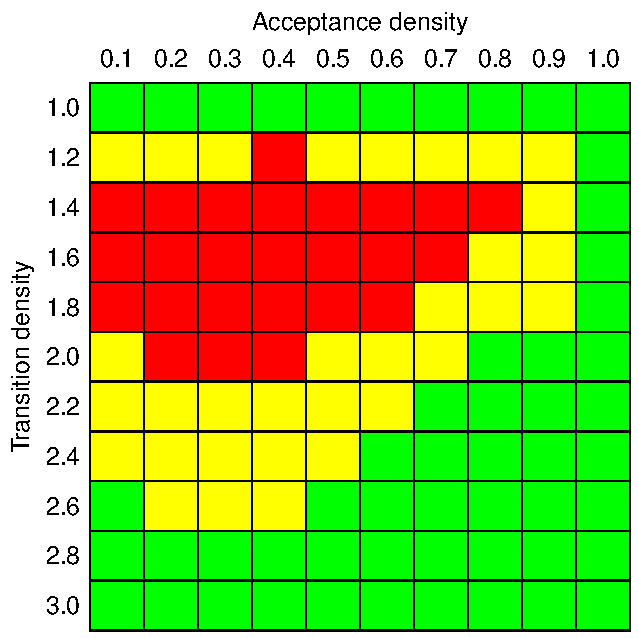
\includegraphics[width=0.4\textwidth]{figures/r/internal/goal/s.median.image.pdf}
\caption{Average of the median number of produced states of all the constructions: green (easy): $\leq$ 500; yellow (medium): $\leq$ 1450; red (hard): $>$ 1450.}
\end{figure}



\subsection{Michel Automata}

\begin{figure}[ht]
  \centering
  \begin{subtable}{0.75\textwidth}
    \centering
    % latex table generated in R 3.1.2 by xtable 1.7-4 package
% Sun Aug 16 00:19:45 2015
\begin{tabular}{lrrrrrr}
  \hline
Construction & Michel 1 & Michel 2 & Michel 3 & Michel 4 & Fitted curve & Std. error \\ 
  \hline
Fribourg & 57 & 843 & 14,535 & 287,907 & $(1.35n)^n$ & 0.01\% \\ 
  Fribourg+R2C & 33 & 467 & 8,271 & 168,291 & $(1.24n)^n$ & 0.06\% \\ 
  Fribourg+M1 & 44 & 448 & 5,506 & 81,765 & $(1.10n)^n$ & 0.07\% \\ 
  Fribourg+M1+M2 & 42 & 402 & 4,404 & 57,116 & $(1.03n)^n$ & 0.12\% \\ 
  Fribourg+M1+M2+R2C & 28 & 269 & 3,168 & 43,957 & $(0.99n)^n$ & 0.04\% \\ 
  Fribourg+R & 18 & 95 & 528 & 3,315 & $(0.64n)^n$ & 0.35\% \\ 
   \hline
\end{tabular}

    \caption{Complement sizes of the first four Michel automata.}
  \end{subtable}

  \begin{subfigure}{0.75\textwidth}
    \centering
    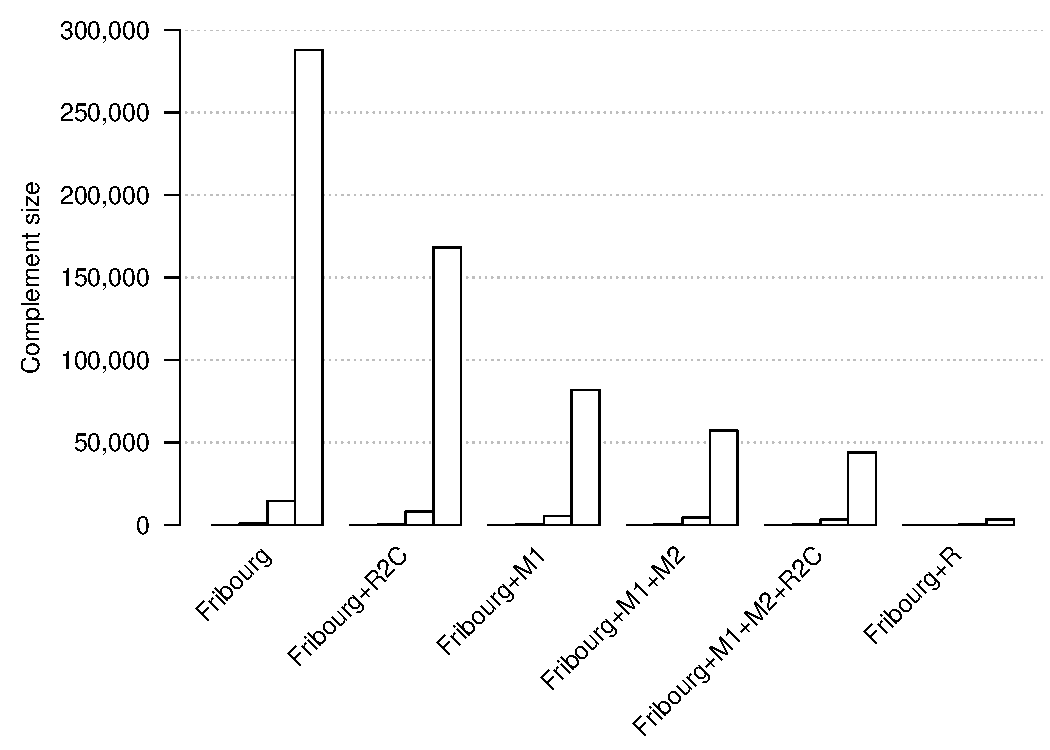
\includegraphics[width=\textwidth]{figures/r/internal/michel/s.barplot.pdf}
    \caption{Complement sizes of the first four Michel visualised as a barplot. The bars 1 to 4 of each group correspond to Michel automata 1 to 4.}
  \end{subfigure}
  \caption{Complement sizes of Michel automata.}
\end{figure}

Michel automata are complete, thus the C options makes no sense.

For the Michel automata Fribourg+M1+M2 is better than Fribourg+M1. Fribourg+M1+R2C is again much better than Fribourg+M1 and even Fribourg+M1+M2. Thus, we have to test Fribourg+M1+M2+R2C. 

\begin{itemize}
\item Add Fribourg+M1+M2+R2C
\item Add Fribourg+M1+M2+R2C+R
\item Add Fribourg+R
\end{itemize}




\section{External Tests}

\subsection{GOAL Test Set}

\begin{table}[ht]
\centering
% latex table generated in R 3.1.2 by xtable 1.7-4 package
% Sat Jun  6 16:42:17 2015
\begin{tabular}{lrr}
  \hline
Construction & Timeouts & Memory excesses \\ 
  \hline
Fribourg & 48 & 0 \\ 
  Fribourg+R2C & 30 & 0 \\ 
  Fribourg+R2C+C & 54 & 0 \\ 
  Fribourg+M1 & 2 & 0 \\ 
  Fribourg+M1+M2 & 1 & 0 \\ 
  Fribourg+M1+R2C & 1 & 0 \\ 
  Fribourg+M1+R2C+C & 8 & 0 \\ 
  Fribourg+R & 48 & 0 \\ 
   \hline
\end{tabular}

\caption{Number of timeouts and memory excesses.}
\end{table}

\begin{itemize}
\item With Rank
  \begin{itemize}
  \item 7,204 effective samples (3,796 uncompleted tasks, 34.51\%)
  \end{itemize}
\item Without Rank
  \begin{itemize}
  \item 10,998 effective samples (2 uncompleted tasks, 0.02\%)
  \end{itemize}
\end{itemize}


\subsubsection{With Rank}

\begin{figure}[ht]
\centering
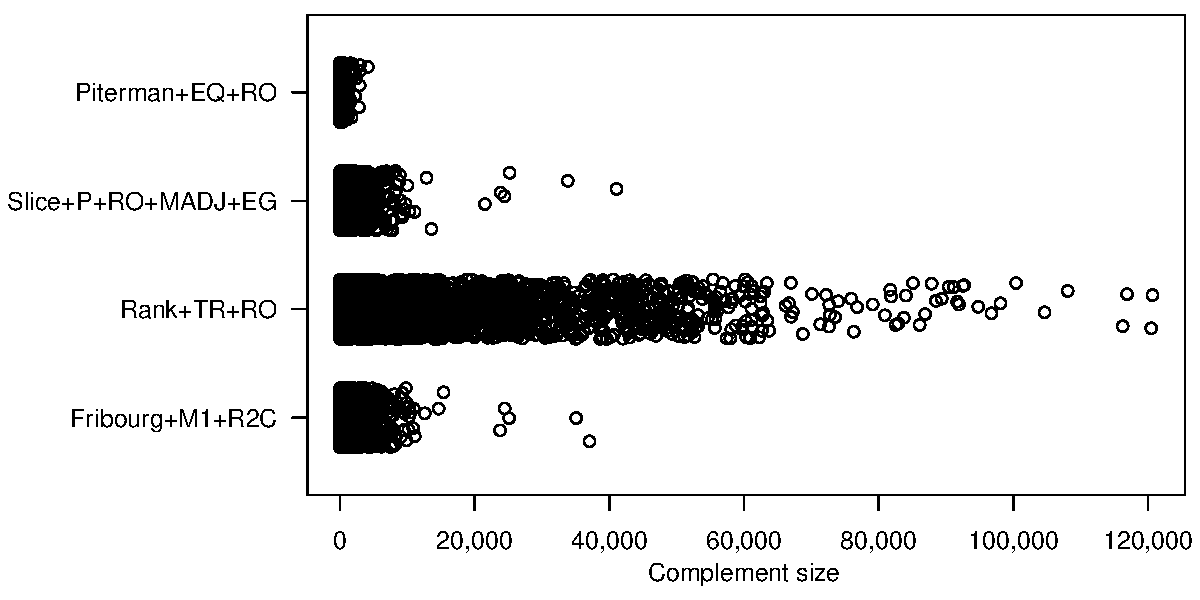
\includegraphics[width=0.75\textwidth]{figures/r/external/goal/s.stripchart.with_rank.pdf}
\caption{Complement sizes of the 7,204 effective samples.}
\end{figure}

\begin{table}[ht]
\centering
% latex table generated in R 3.1.2 by xtable 1.7-4 package
% Sun Aug 16 15:57:19 2015
\begin{tabular}{lrrrrrr}
  \hline
Construction & Mean & Min. & P25 & Median & P75 & Max. \\ 
  \hline
Piterman+EQ+RO & 106.0 & 1 & 29.0 & 58.0 & 121.0 & 4,126 \\ 
  Slice+P+RO+MADJ+EG & 555.4 & 2 & 70.0 & 202.0 & 596.0 & 41,081 \\ 
  Rank+TR+RO & 5,255.6 & 2 & 81.0 & 254.5 & 3,178.2 & 120,674 \\ 
  Fribourg+M1+R2C & 662.9 & 2 & 101.0 & 269.0 & 754.5 & 37,068 \\ 
   \hline
\end{tabular}

\caption{Aggregated statistics of complement sizes of the 7,204 effective samples.}
\end{table}

\begin{table}[ht]
\centering
% latex table generated in R 3.1.2 by xtable 1.7-4 package
% Thu Jun 11 15:11:29 2015
\begin{tabular}{lrrrrrr}
  \hline
Construction & Mean & Min. & P25 & Median & P75 & Max. \\ 
  \hline
Piterman+EQ+RO & 2.97 & 2.22 & 2.58 & 2.78 & 3.03 & 42.93 \\ 
  Slice+P+RO+MADJ+EG & 3.66 & 2.21 & 2.69 & 3.22 & 4.07 & 36.67 \\ 
  Rank+TR+RO & 16.04 & 2.28 & 2.76 & 3.71 & 9.31 & 443.33 \\ 
  Fribourg+M1+R2C & 4.02 & 2.22 & 2.69 & 3.10 & 4.37 & 410.37 \\ 
   \hline
\end{tabular}

\caption{Aggregated statistics of the running times of the 7,204 effective samples.}
\end{table}


\subsubsection{Without Rank}


\begin{figure}[ht]
\centering
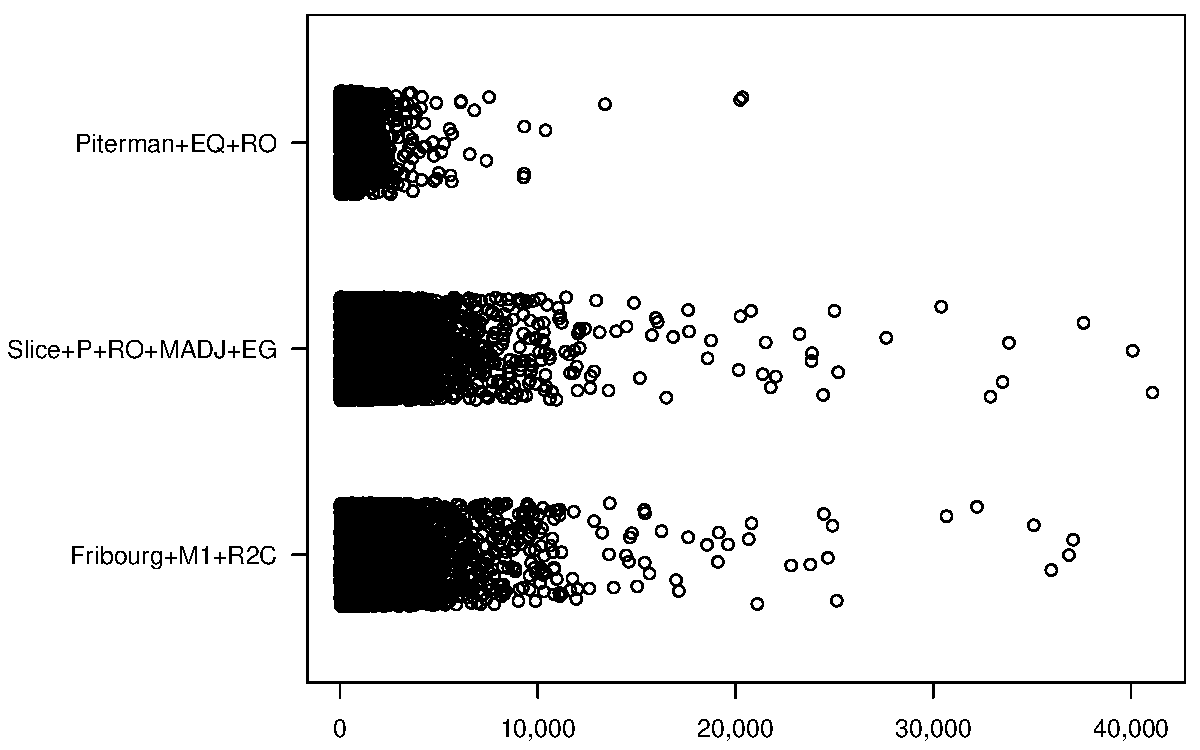
\includegraphics[width=0.75\textwidth]{figures/r/external/goal/s.stripchart.pdf}
\caption{Complement sizes of the 10,998  effective samples.}
\end{figure}


\begin{table}[ht]
\centering
% latex table generated in R 3.1.2 by xtable 1.7-4 package
% Sat Jun  6 16:42:20 2015
\begin{tabular}{lrrrrrr}
  \hline
Construction & Mean & Min. & P25 & Median & P75 & Max. \\ 
  \hline
Piterman+EQ+RO & 209.6 & 1 & 38.0 & 80.0 & 183.0 & 20,349 \\ 
  Slice+P+RO+MADJ+EG & 949.4 & 2 & 120.0 & 396.0 & 1,003.0 & 41,081 \\ 
  Fribourg+M1+R2C & 1,017.3 & 2 & 153.0 & 452.0 & 1,134.0 & 37,068 \\ 
   \hline
\end{tabular}

\caption{Aggregated statistics of complement sizes of the 10,998 effective samples without Rank.}
\end{table}

\begin{table}[ht]
\centering
% latex table generated in R 3.1.2 by xtable 1.7-4 package
% Wed Aug 19 09:24:28 2015
\begin{tabular}{LrrrrrrRr}
  \hline
Construction & Mean & Min. & P25 & Median & P75 & Max. & Total & $\approx$ hours \\ 
  \hline
Fribourg & 8.5 & 2.5 & 3.3 & 4.9 & 7.3 & 586.0 & 93,351.2 & 259 \\ 
  Fribourg+R2C & 6.6 & 2.2 & 2.9 & 4.2 & 6.4 & 219.7 & 72,545.7 & 202 \\ 
  Fribourg+R2C+C & 8.5 & 2.2 & 2.6 & 3.5 & 6.4 & 582.9 & 93,396.2 & 259 \\ 
  Fribourg+M1 & 4.9 & 2.5 & 3.2 & 4.1 & 5.9 & 55.1 & 54,061.3 & 150 \\ 
  Fribourg+M1+R2C & 4.4 & 2.2 & 2.8 & 3.6 & 5.3 & 42.5 & 48,572.0 & 135 \\ 
  Fribourg+M1+R2C+C & 5.6 & 2.5 & 3.2 & 4.0 & 6.5 & 147.4 & 60,918.9 & 169 \\ 
  Fribourg+M1+M2 & 4.6 & 2.2 & 2.9 & 3.8 & 5.1 & 38.4 & 49,848.0 & 138 \\ 
  Fribourg+R & 7.5 & 2.2 & 3.0 & 3.9 & 6.3 & 470.5 & 82,387.3 & 229 \\ 
   \hline
\end{tabular}

\caption{Aggregated statistics of the running times of the 10,998 effective samples without Rank.}
\end{table}

% Persp plots
\renewcommand{\perspwidth}{0.3}

\begin{figure}[ht]
\centering
  \hfill
  \begin{subfigure}[t]{\perspwidth\textwidth}
  \centering
  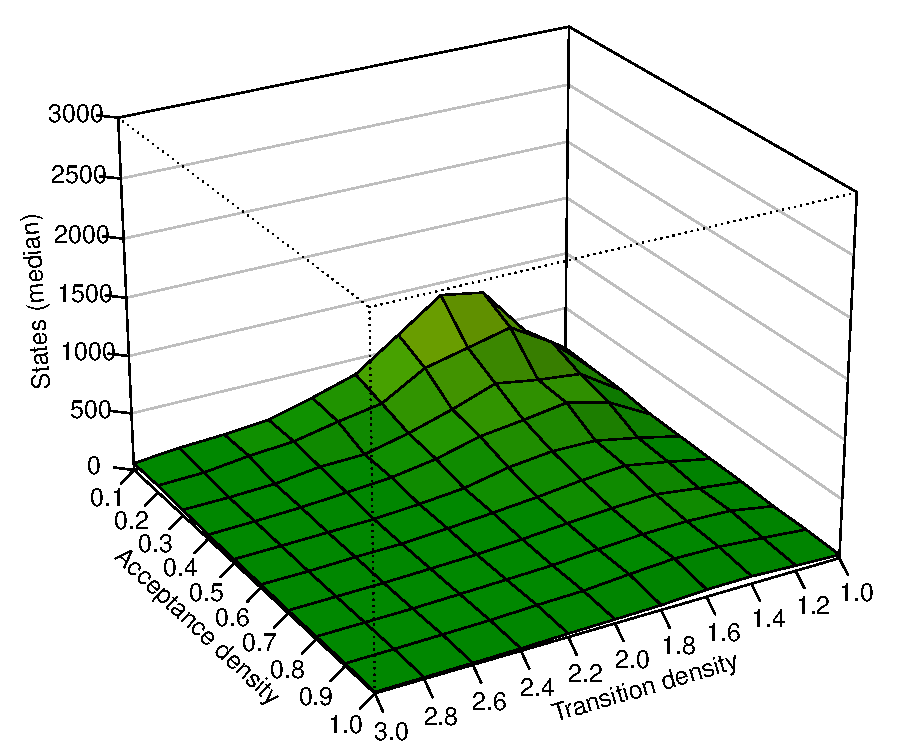
\includegraphics[width=\textwidth]{figures/r/external/goal/s.median.Piterman+EQ+RO.pdf}
  \caption{Piterman+EQ+RO}
  \end{subfigure}
  \hfill
  \begin{subfigure}[t]{\perspwidth\textwidth}
  \centering
  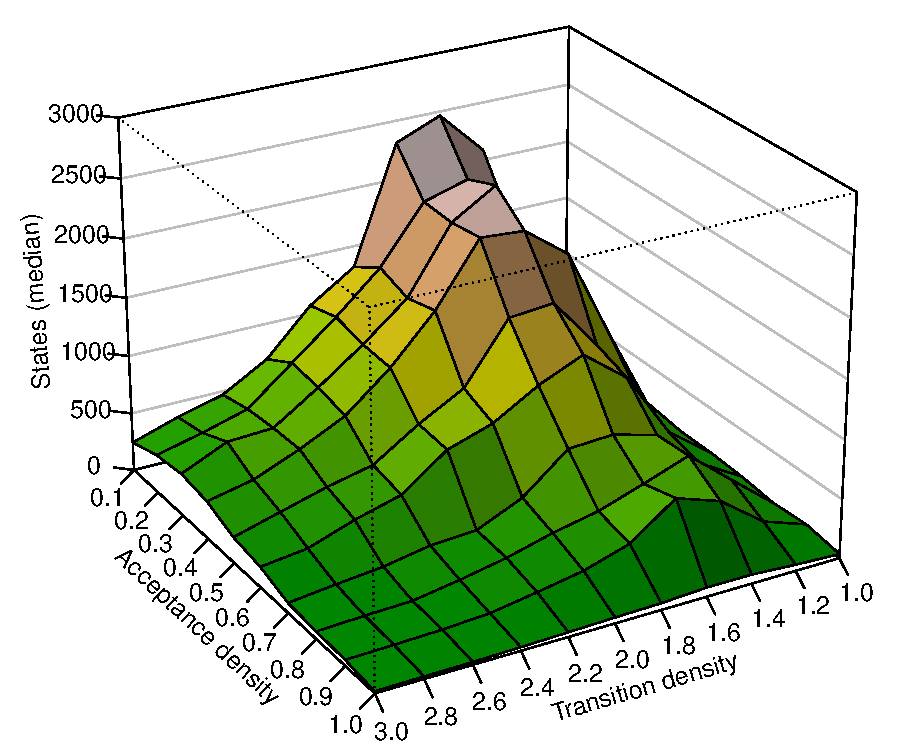
\includegraphics[width=\textwidth]{figures/r/external/goal/s.median.Slice+P+RO+MADJ+EG.pdf}
  \caption{Slice+P+RO+MADJ+EG}
  \end{subfigure}
  \hfill
  \begin{subfigure}[t]{\perspwidth\textwidth}
  \centering
  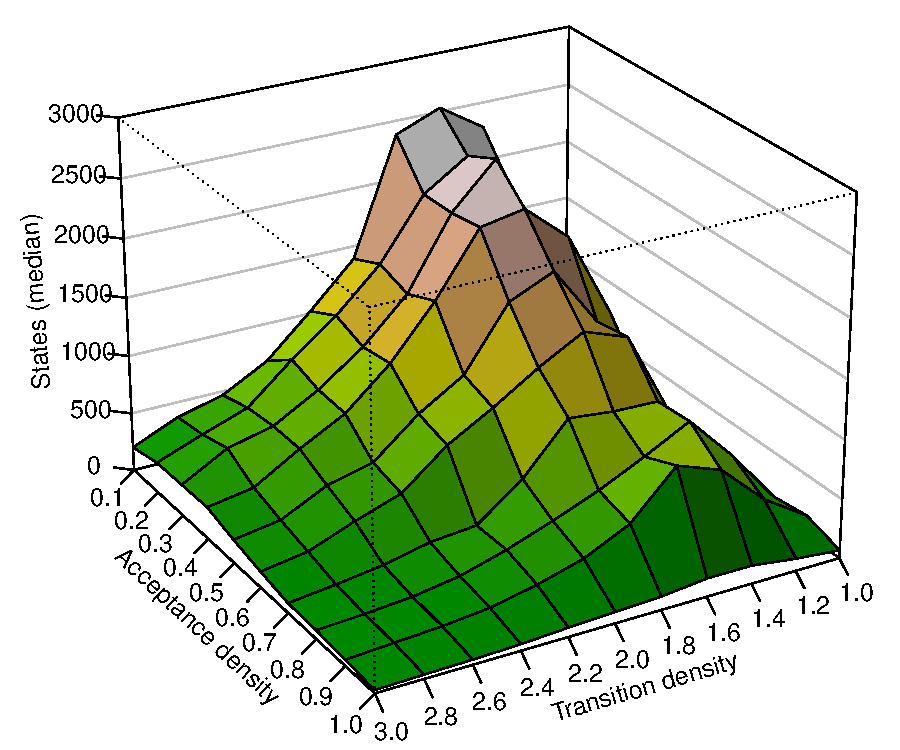
\includegraphics[width=\textwidth]{figures/r/external/goal/s.median.Fribourg+M1+R2C.pdf}
  \caption{Fribourg+M1+R2C}
  \end{subfigure}
  \hfill
\caption{Median complement sizes.}
\end{figure}



\subsection{Michel Automata}


\begin{figure}[ht]
  \centering
  \begin{subtable}{0.75\textwidth}
    \centering
    % latex table generated in R 3.1.2 by xtable 1.7-4 package
% Sun Aug 16 00:19:45 2015
\begin{tabular}{lrrrrrr}
  \hline
Construction & Michel 1 & Michel 2 & Michel 3 & Michel 4 & Fitted curve & Std. error \\ 
  \hline
Fribourg & 57 & 843 & 14,535 & 287,907 & $(1.35n)^n$ & 0.01\% \\ 
  Fribourg+R2C & 33 & 467 & 8,271 & 168,291 & $(1.24n)^n$ & 0.06\% \\ 
  Fribourg+M1 & 44 & 448 & 5,506 & 81,765 & $(1.10n)^n$ & 0.07\% \\ 
  Fribourg+M1+M2 & 42 & 402 & 4,404 & 57,116 & $(1.03n)^n$ & 0.12\% \\ 
  Fribourg+M1+M2+R2C & 28 & 269 & 3,168 & 43,957 & $(0.99n)^n$ & 0.04\% \\ 
  Fribourg+R & 18 & 95 & 528 & 3,315 & $(0.64n)^n$ & 0.35\% \\ 
   \hline
\end{tabular}

    \caption{Complement sizes of the first four Michel automata.}
  \end{subtable}

  \begin{subfigure}{0.75\textwidth}
    \centering
    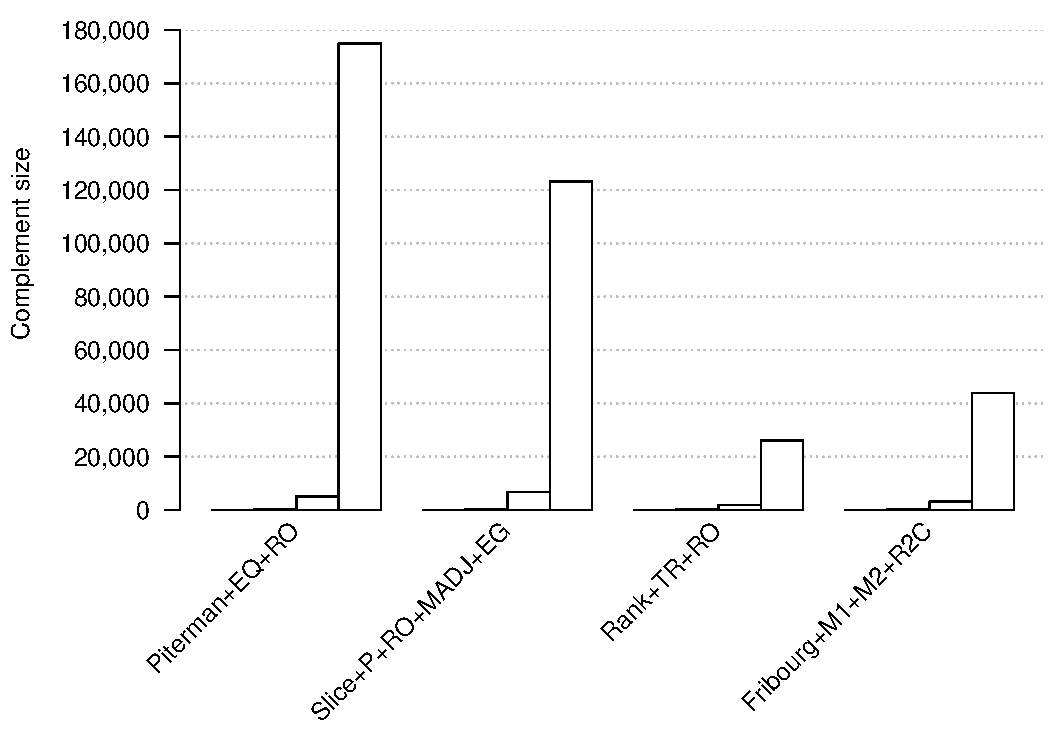
\includegraphics[width=\textwidth]{figures/r/external/michel/s.barplot.pdf}
    \caption{Complement sizes of the first four Michel visualised as a barplot. The bars 1 to 4 of each group correspond to Michel automata 1 to 4.}
  \end{subfigure}
  \caption{Complement sizes of Michel automata.}
\end{figure}


\begin{table}[ht]
\centering
% latex table generated in R 3.1.2 by xtable 1.7-4 package
% Sun Aug 16 00:19:45 2015
\begin{tabular}{lrrrrrr}
  \hline
Construction & Michel 1 & Michel 2 & Michel 3 & Michel 4 & Fitted curve & Std. error \\ 
  \hline
Fribourg & 57 & 843 & 14,535 & 287,907 & $(1.35n)^n$ & 0.01\% \\ 
  Fribourg+R2C & 33 & 467 & 8,271 & 168,291 & $(1.24n)^n$ & 0.06\% \\ 
  Fribourg+M1 & 44 & 448 & 5,506 & 81,765 & $(1.10n)^n$ & 0.07\% \\ 
  Fribourg+M1+M2 & 42 & 402 & 4,404 & 57,116 & $(1.03n)^n$ & 0.12\% \\ 
  Fribourg+M1+M2+R2C & 28 & 269 & 3,168 & 43,957 & $(0.99n)^n$ & 0.04\% \\ 
  Fribourg+R & 18 & 95 & 528 & 3,315 & $(0.64n)^n$ & 0.35\% \\ 
   \hline
\end{tabular}

\caption{Execution times for the first four Michel automata.}
\end{table}
